\chapter{Conception of the DO}

The DO is a solution to the problem of distributed data acquisition. It takes advantage of the knowledge gathered by other people while creating distributed systems (chapter 2), and modern technologies which are currently available (chapter 3).
A deep study of existing solutions and a proper choice of the technologies are fundamental in achieving the goal of the distributed data acquisition in an efficient way.

In order to fulfil this goal, the following fundamental questions had to be answered:
\begin{itemize}
    \item How to make sure that the data from various devices corresponds to the same moment in time?
    \item What should the architecture of the system be?
    \item How to establish communication between the nodes?
\end{itemize}
These questions are answered in this chapter. The implementation details are described in the following chapter.

\section{Data synchronisation} \label{section:data_synchronisation}
    As it is explained in section \ref{section:WRTD}, WRTD allows distributing the triggers with known delay. However, even though the time of the trigger and the value of the delay are known, it does not mean that the devices are triggered at the same time. While acquiring the synchronised data, it is desirable that the data correspond to the same moment in time. In order to achieve this, DO uses the WRTD project to distribute the triggers, modifies the acquisition settings of the ADCs and processes the acquired data in order to align it.
    
    The idea of this operation is presented in Fig. \ref{fig:DO_pre_post}. Since the delay between the triggers of the ADCs is known, the acquired pre-samples and post-samples\footnote{The arrow of post-samples pointing to the left means the negative value of the post-samples, which in this situation specifies the number of samples that are NOT acquired before the trigger. In the actual hardware, it is not possible to set a negative value of post-samples, therefore it is set to 0 and the acquired data is truncated.} (the samples that are acquired before and after the trigger accordingly), could be configured to compensate for the delay between the triggers. 
    
    \begin{figure}
    	\centerline{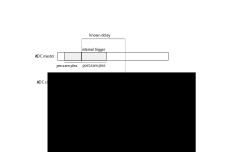
\includegraphics[width=0.7\textwidth]{figures/DO_pre_post.pdf}}
    	\caption{Configuration of pre-samples and post-samples in the DO}
    	\label{fig:DO_pre_post}
    \end{figure}
    
    In order to achieve this, two types of ADC configurations have been distinguished:
    \begin{itemize}
        \item master's ADC configuration --- the ADC which is triggered internally and distributes WRTD timestamps,
        \item slave's ADC configuration --- the ADC that is triggered by WRTD timestamps.
    \end{itemize}
    
    The user configures the master ADC the way he would configure a standard ADC, selecting the number of pre-samples and post-samples that he wants to acquire --- these values directly translate into the horizontal scale in the standard oscilloscope. 
    
    The slave ADCs have to be configured to return the data corresponding to the time of the trigger of the master ADC. For this purpose, the value of pre-samples and post-samples should be calculated according to the equations \ref{eq:pre-samples} and \ref{eq:post-samples}.
    
    \begin{equation}\label{eq:pre-samples}
        \text{pre-samples} = \text{pre-samples}_\text{required} + \Delta t * f_s
    \end{equation}
    
    \begin{equation} \label{eq:post-samples}
        \text{post-samples} = \text{post-samples}_\text{required} - \Delta t * f_s
    \end{equation}
    $\Delta t$ --- the known delay between the triggers,\\
    $f_s$ --- the sampling frequency of the ADC.
    
    With these settings, the number of samples that are acquired before and after the original trigger in each ADC is the same, therefore the data correspond to the same moment in time, even though the actual devices were triggered at different moments.
    
\section{General architecture} \label{section:general_architecture}
    When designing a distributed system, the question of architecture is fundamental. The choice of the architecture at the first phase of the project has a strong influence on all stages of the design, as well as the maintenance after deployment. That is why a lot of attention was devoted to this matter.
    
    There are two ways of connecting clients with each other. The first is to connect each device to each user, presented in Fig. \ref{fig:DO_schem_no_proxy}. The second option is to create a proxy that has the information about all the users and all the devices, presented in Fig. \ref{fig:DO_schem_proxy}. In the thesis, this proxy is called the DO Server. In case of using the term server e.g. in the RPC, it is explicitly stated. The Front End Computer (FEC) is a machine in which the ADC card is installed.

    \begin{figure}
    	\centerline{\includegraphics[width=0.7\textwidth]{figures/DO_basic_schematics_no_proxy.pdf}}
    	\caption{Connection of clients and devices without proxy}
    	\label{fig:DO_schem_no_proxy}
    \end{figure}
    
    \begin{figure}
    	\centerline{\includegraphics[width=0.7\textwidth]{figures/DO_basic_schematics.pdf}}
    	\caption{Connection of clients and devices using proxy}
    	\label{fig:DO_schem_proxy}
    \end{figure}
    
    The advantages of the design with the DO Server are the following:
    \begin{itemize}
        \item The system is divided into more smaller applications. It is easier to manage the code and upgrade its parts. However, the same result could be obtained designing the application properly in a modular way, yet for a inexperienced developer, such architecture enforces more careful design.
        \item In case of a design without the DO Server, some part of the code would have to be moved to the ADC application, which should be as lightweight as possible. The ADC application should be lightweight, because it may be run on a machine with little processing power, which serves uniquely as a host.
        \item In case of bigger networks, such a configuration is much easier to manage.
        \item If the DO is developed into a bigger system, the centralised unit having knowledge of all the connections could allow implementing algorithms optimising the access to the devices. However, at this moment, no such algorithm is implemented.
        \item The GUI module could be easily replaced with another application, not necessarily requiring plotting the data and having the graphical interface.
        \item Having a centralised unit eases the service discovery --- when adding a new device to the system, the address of just one element has to be known.
    \end{itemize}
    Counterarguments of using proxy are the following:
    \begin{itemize}
        \item Adding a proxy introduces some overhead in the communication between the user and the ADC.
        \item Adding a proxy introduces another abstraction layer, which could make the design unnecessarily more complicated in case of a small system. 
    \end{itemize}
    
    Taking into account all the arguments, the version with the DO Server was chosen. This choice has complicated the first stage of the design, however, the choice has proved to be good while testing the application and performing the measurements.
    
    The implementation details of various DO components are described in the following chapter.

\section{Communication} \label{section:communication}

    When designing a distributed system, apart from the general architecture, the other fundamental aspect is how the nodes communicate with each other. After analysis of the DO requirements, the following aspects of communication were pointed out:
    \begin{itemize}
        \item Enumeration of devices and establishing the connection. 
        \item Control of the run-time behaviour of nodes by the GUI.
        \item Transmission of the acquisition data and notifications.
    \end{itemize}
    The schematic of communication used in the DO is presented in Fig. \ref{fig:DO_communication}. The mentioned points are explained in more detail in the following sections.
    \begin{figure}
    	\centerline{\includegraphics[width=\textwidth]{figures/DO_communication.pdf}}
    	\caption{Schematic of communication in the DO}
    	\label{fig:DO_communication}
    \end{figure}

    \subsection{Enumeration of the devices} \label{section:enumeration_of_devices}
        %Solution in DO
        %Introduction
        In order to ease the connection of new devices, it was decided that they should be discovered automatically by the DO Server. The other reason for this choice was to make the DO compatible with the LXI. The library chosen for that purpose was Python-Zeroconf, described in section~\ref{subsec:zeroconf}. Since there was no strict requirement for this particular technology, the choice of the library was based on its popularity.
        
        %How is it implemented
        The zeroconf listener runs on the DO Server. The ADCs, when connected to the network, advertise themselves. When the DO Server discovers a new device whose name suits the predefined restrictions, it starts the communication.
        
        This solution works correctly only as long as the devices are in the same local network. However, taking into account the fact that the DO is a distributed system, it cannot be assured that all the devices will be in the same local network. For this reason, two connection mechanism where implemented:
        \begin{itemize}
            \item Connection using zeroconf.
            \item Manual configuration.
        \end{itemize}
        If the server address is provided during the startup of the ADC application, the device connects to this address. Otherwise, it uses the previously described method.
    
    \subsection{Control of the run-time behaviour of the nodes} \label{section:run_time_beh}
        
        %reason for the RPC
        In order to control the run-time behaviour by the GUI, the RPC is used. This choice was made at the moment of selecting the architecture of the system: the main reason not to select the architecture with the DO Server was that it complicates the design. However, the use of the RPC was considered to make writing a distributed application in some way similar to writing a stand-alone application. Therefore, the choice of the architecture with the DO Server, together with the use of the RPC was considered the optimal solution, combining the advantages of the DO Server and reducing its greatest disadvantage --- the complexity.
        
        %data flow
        The distribution of the RPC servers and clients, presented in Fig. \ref{fig:DO_communication}, is based on the fact that the GUI is the node that controls the behaviour of the DO Server, and the DO Server controls the behaviour of the ADCs. There is no reason for the DO Server to issue an RPC to the GUI, therefore there is no RPC server in the GUI. The same applies for the ADC and the DO Server.
        
        At the beginning of the development of the DO, the communication scheme was not particularly well planned and the RPC servers were located in each of the nodes of the system. It caused issuing the nested RPCs, which at some point were blocking the entire application. This situation was a proof that the previous statement that \textit{the use of the RPC makes writing the distributed applications in some way similar to monolithic applications} was wrong.
        
        The implementation details and the choice of the RPC is described in more detail in the following chapter.
        
    \subsection{Transmission of acquired data and notifications} \label{section:transmission_data_notifications}
        RPCs are used for the majority of the communication between the modules except for three cases when there is an asynchronous event on the device side:
        \begin{itemize}
            \item acquired data
            \item notifications about the presence of the new device
            \item notifications about the availability of the device (in case it is used by different application)
        \end{itemize}
        
        When sending this information, there is no need for the callback, therefore one way communication is used. 
        For that purpose, the publisher/subscriber pattern is chosen, in which the publisher sends the asynchronous data to the subscriber. 
        
        In case of acquiring large arrays of data, this part of communication is the most crucial when optimising the speed of data acquisition. For that reason, various tools were evaluated in order to provide high speed and reliable data acquisition. The comparison of these tools is presented in section \ref{section:acquisition_speed_optimisation}.\\

    
    
    
     This chapter described the fundamental aspects considered when creating a system for a distributed data acquisition. The implementation details of the DO are described in the following chapter.
